Las técnicas de evaluación , como se comentó en la sección de los datasets son relevantes para verificar las capacidades del modelo y de las características que han definido el proceso de entrenamiento de este.
En este sentido, se suelen utilizar métricas que indican estas capacidades, como por ejemplo la precisión, la exactitud, el recall o la F1-score. Estas métricas permiten evaluar el rendimiento del modelo en términos de capacidad para clasificar correctamente los datos, identificar verdaderos positivos y negativos, y equilibrar la precisión y el recall.
Además, es importante considerar la matriz de confusión, que proporciona una representación visual de los resultados de clasificación, mostrando las verdaderas clases frente a las predichas por el modelo. Esto ayuda a identificar patrones de error y áreas donde el modelo puede estar fallando.

\begin{figure}[H]
    \begin{center}
    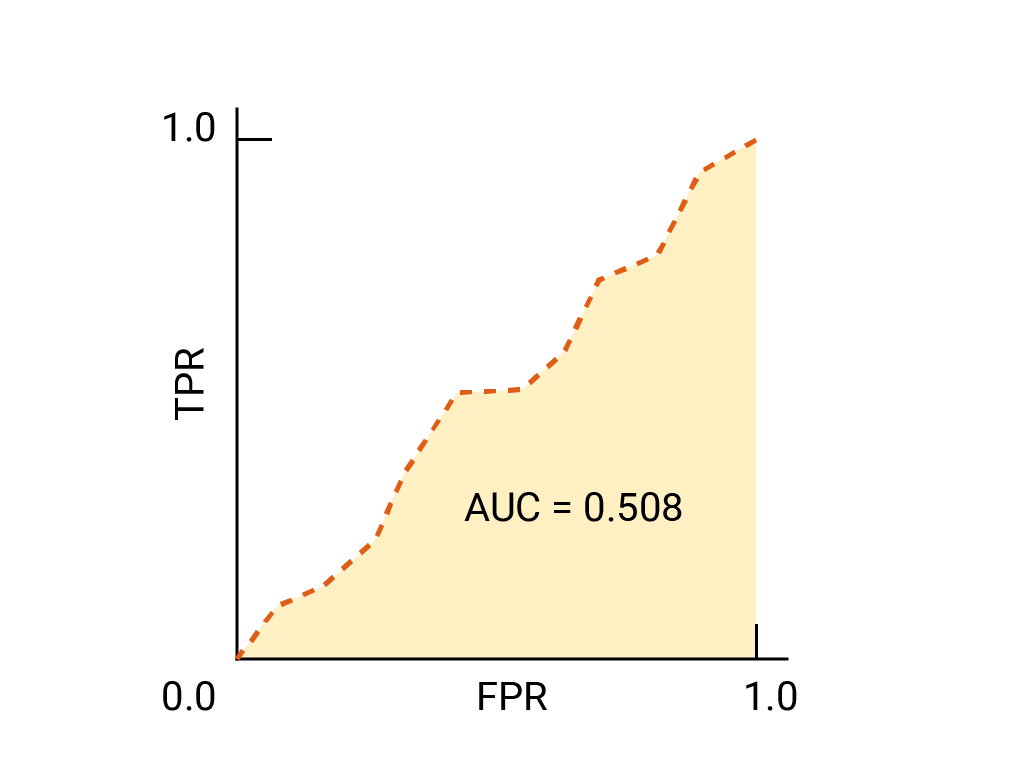
\includegraphics[width=0.7\textwidth]{commons/Fig8.png}
    \caption{Ejemplo de graficación de la métrica AUC. Esta métrica parte de la matriz de confusión generando un gráfico de puntos donde 
    se evalúa la capacidad del modelo para clasificar correctamente en función de los valores por debajo de la diagonal del gráfico.}
    \label{fig:AUC}
    \cite{rafii18}
    \end{center}
\end{figure}

Algunas métricas:

\begin{itemize}
    \item SI-SDR: mide la fidelidad de un sonido estimado en comparación con un audio de referencia.
    \item SDR/SAS/SIS: miden la relación señal-distorsión,señal-ruido presente,y señal-interferencia  respectivamente.
    \item Media: medida de tendencia central
    \item Mediana: valor central en datos ordenados.
    \item Desviación típica: indica cuanto se aleja en promedio un conjunto de valores respecto a su media.
\end{itemize}